\section{Experiments and results}
The data come from the MNIST dataset, containing 60000 train images and 10000 test images from 10 almost balanced classes (arabic numerals). The following simulations generate a universal adversarial perturbation starting from a portion of the MNIST train dataset. Then the perturbation is added to the test images that have been correctly classified by the pre-trained LeNet-5 convolutional neural network, aiming to maximally increase the loss function, and therefore minimize the accuracy.\\
In particular, the perturbation has to inject a minimal visual distortion to the original images and this is ensured by the constraint on the $\ell_{\infty}$ norm in the optimization problem (1). Therefore, the digits in the perturbed images still appear clearly distinguishable to the human eyes, but get misclassified by LeNet5.\\
In the following experiments, the $\ell_{\infty}$ norm of the perturbation is chosen so as not to be higher than $\varepsilon=0.25$.\\

For semplicity, all the algorithms introduced in the previous section have been implemented in a sequential fashion, rather than using a proper distributed architecture. Therefore, the workers do not effectly represent different processors in different machines, but they are just different methods called by the same machine, imitating a distributed setting. Nevertheless, all the algorithms can be easily modified to accomodate a proper distributed architecture by configuring Ray\footnote{Ray: https://github.com/ray-project/ray.} or PySpark\footnote{PySpark: https://spark.apache.org/docs/latest/api/python.}.\\

Again, for semplicity, the algorithms do not involve a normalization tecnique for the perturbed images and therefore normalization has been applied only after the computation of the universal adversarial perturbation, that is just before the testing of LeNet5. A possible improvement could be to consider the Box constraint described in \cite{A1}, section V.B.\\

In addition, a key concept of the Frank-Wolfe theory is the duality gap, that is an upper bound for the primal suboptimality $F(x_t)-F(x^*)$ defined as:
\begin{equation}
	\mathcal{G}(\mathbf{x}) =\max_{\mathbf{s}\in\mathit{C}} \langle \nabla F(\mathbf{x}),\mathbf{x}-\mathbf{s}\rangle.
\end{equation}
Therefore, a further improvement of the implementation could be the use of the Frank-Wolfe duality gap as stopping criterion for the algorithms. However, this turned out to be difficult in the distributed settings at hand.

\subsection{Decentralized Stochastic Gradient Free Frank Wolfe}
\textcolor{blue}{Usiamo il passato ora, siccome e` un esperimento svolto}
To study the performance of Algorithm \ref{decentralized} we used the 10000 images in the MNIST test set, after normalizing them.\\ We split the digit images by giving 10 samples of each class to our 10 workers. In such way, we make each worker holding a hundred images. After tuning the hyperparameter $m$ of the number of direction, we discovered that $m=15$ was the good compromise between the computation time and the overall results. For each image we estimated its gradient using 20, 50 and 100 queries.

\textcolor{gray}{Accuracy error achieved, during the training of the model, the we need to compare the result achieved by testing the model on the whole test set.\\ Notice that the drop of the accuracy, hence the accuracy is discovered already at the 10 epoch/iteration of the algorithms. Comparing the three algorithm is almost the faster one, the competing algorithm in terms of speed convergence of the noise is the distributed.
\\ presence of the pattern in the noise when the accuracy is minimized, more is minimized more the noise the pattern is visible in this algorithms. INstead in the other algorithms the pattern is less visibile e secondo silvia per esempio il variance reduced non presenta un pattern appunto perche il noise e` piu distribuito siccome per la proprieta della varianza considerata nell'algoritmo.
Un piccolo confronto con il guassian noise come fatto nel jupyter sarebbe il top.
}
\begin{figure}[htbp]
	\centering
	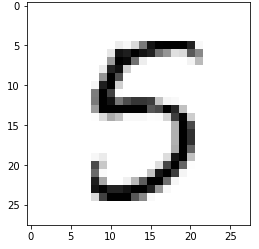
\includegraphics[width=3.6cm]{real_image_5.png}\hfil
	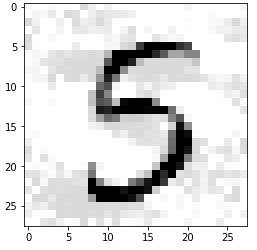
\includegraphics[width=3.58cm]{report_decentralized_T50_m15.png}
	\caption{Image of 5 changed to 3 with the adversarial perturbation generated by the Decentralized Algorithm \ref{decentralized} with a query of 50 and 15 directions.}
	\label{fig:decentralized}
\end{figure}
In Figure \ref{fig:decentralized} we can see an example of the perturbation applyed on an image of the MNIST digits.

\subsection{Decentralized Variance-Reduced Stochastic Gradient Free Frank Wolfe}
For the Variance-Reduced FW algorithm we consider 5 workers and with 800 different images each, i.e. 160 images per digit. We set the number of queries to 20 and the number of component functions $S_2 = 3$. We then run the Algorithm \ref{variance-reduced} for $q=5,7,9$ and $n=5,10$. The choice for the values of $q$ is because of the different number of calling to the KWSA, while the $n$ parameter identify the different number of component function.\\

DA SPIEGARE MEGLIO, QUESTA PARTE NON L'AVEVO CAPITA MOLTO BENE :(

\begin{figure}[htbp]
	\centering
	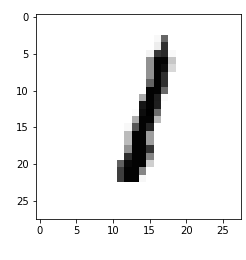
\includegraphics[width=3.7cm]{real_image.png}
	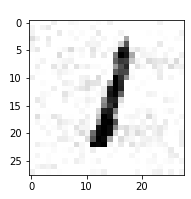
\includegraphics[width=3.9cm]{perturbed_images.png}
	\caption{Perturbation and perturbed image of the distributed FW with T=100 and m=15.}
	\label{fig:variance-reduced}
\end{figure}
In Figure \ref{fig:variance-reduced} we can see an example of the perturbations.


\subsection{Distributed Stochastic Gradient Free Frank Wolfe}
To test the performance of Algorithm \ref{distributed} we used 10 workers and an adjacecy matrix $A$ given by 
\[ A = 
\begin{pmatrix}
1& 1& 0& 1& 1& 1& 1& 1& 0& 1\\
1& 1& 1& 0& 1& 1& 1& 0& 1& 1\\
0& 1& 1& 1& 1& 1& 0& 1& 1& 1\\
1& 0& 1& 1& 1& 1& 0& 1& 1& 1\\
1& 1& 1& 1& 1& 1& 1& 0& 1& 1\\
1& 1& 1& 1& 1& 1& 1& 1& 1& 0\\
1& 1& 0& 0& 1& 1& 1& 1& 1& 1\\
1& 0& 1& 1& 0& 1& 1& 1& 1& 1\\
0& 1& 1& 1& 1& 1& 1& 1& 1& 1\\
1& 1& 1& 1& 1& 0& 1& 1& 1& 1	
\end{pmatrix}
.\]
We can notice that the diagonal is of ones, this because each node is connected to itself. Our network is composed of 10 nodes and the connectivity of the graph can be know by computing $\Vert W- J \Vert$, where $J= 11^T/10$ and $11^T$ represent a matrix with all entries set to 1. In our case we have a connectivity value of 0.438. We use 15 directions and test the algorithm for 20, 50 and 100 queries.

\begin{figure}[htbp]
	\centering
	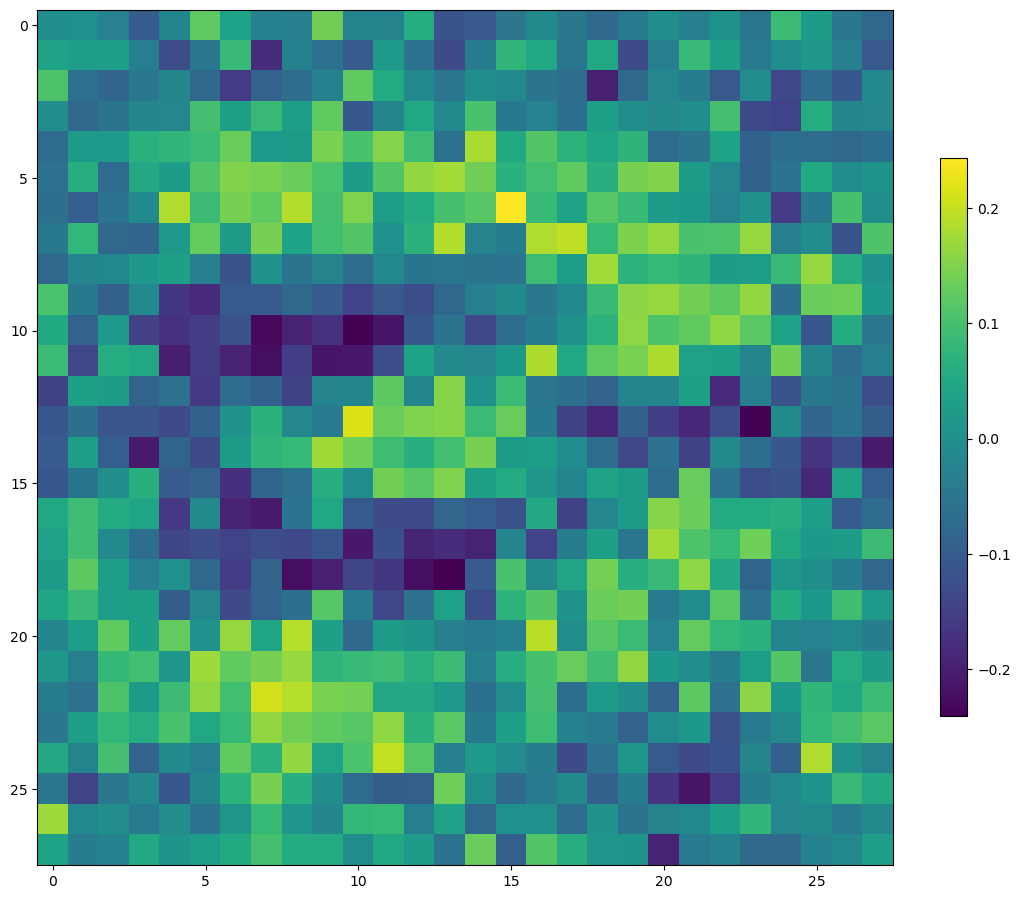
\includegraphics[width=4cm]{report_distributed_delta_20_15.png}
	\caption{Perturbation generated by the Distributed Algorithm \ref{distributed} with a query of 20 and 15 directions.}
	\label{fig:variance-reduced}
\end{figure}

\subsection{Comparison between the perturbations}
